%The \lhcb collaboration has published many interesting results involving a \decay{b}{s\mumu} FCNC,
%many of these involve the decay
%\decay{B}{K\mumu}~\cite{LHCb-PAPER-2012-024,LHCb-PAPER-2012-021,LHCb-PAPER-2012-011}.
%transisiton with a spectator quark, and then the decay of the \Kstar.

%Recently there has been much interest surrounding an observed $3.7\stdev$ deviation from
%theoretial predictions in the value of an observable in the angular distribution of the decay
%\decay{\Bd}{\Kstarent\mumu}~\cite{LHCb-PAPER-2013-037}.
%This decay proceeds via a \decay{\bquark}{\squark\mumu} FCNC where the other quark in the $B$ meson
%is a spectator.
%Analagous diagrams are possible, whereby additional quarks contribute to the final state
%forming either a $\kpipi\mumu$ or $\phik\mumu$ system.
%Figure~\ref{fig:hhh:feyn} shows ways that these final states might be formed from decaying $B$
%mesons.

%These final states have added challenges because they result from the decay of numerous strange
%resonances.

%\begin{figure}
  %\begin{center}
    %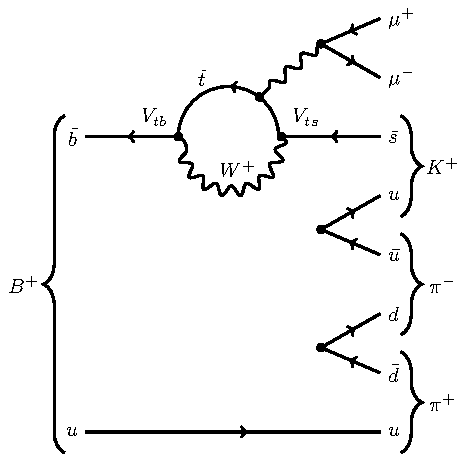
\includegraphics[scale=1]{feynman_hhh_kpipimumu}
    %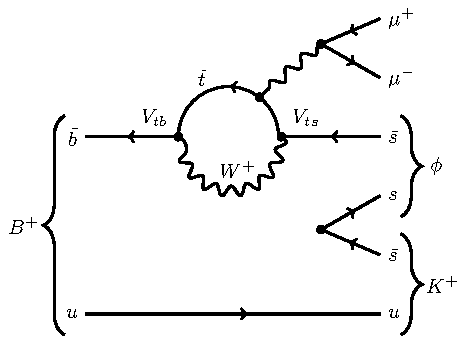
\includegraphics[scale=1]{feynman_hhh_phikmumu}
    %\caption[Feynman diagrams for \btokpipimumu and \btophikmumu]
    %{\small
      %Feynman diagrams illustrating how the decays \btokpipimumu and \btophikmumu can proceed in
      %the SM.
    %}
    %\label{fig:hhh:feyn}
  %\end{center}
%\end{figure}

%This has additional interest in that, not only does it probe the FCNC, but the \kpipi system can
%result from the decay of numerous strange resonances.

The decays \btokpipimumu and \btophikmumu both proceed via \decay{\bquark}{\squark\mumu} FCNC
transitions, which are forbidden at tree level in the \sm.
Therefore, these processes are potentially sensitive to virtual \np particles contributing
to the decay amplitude in loops.
%Figure~\ref{fig:hhh:feyn} shows the pengiun diagrams which propagate these decays in the SM.


%%%%%%%%%%%%%%%%%%%%%%%%%%%%%%%%%%%%%%%%%%%%%%%%%%%%%%%%%%%%%%%%%%%%%%%%%%%%%%%%%%%%%%%%%%%%%%%%%%
%\subsection[Operator product expansion for \btokpipimumu and \btophikmumu]
%{Operator product expansion for $\boldsymbol{\btokpipimumu}$ and $\boldsymbol{\btophikmumu}$}
%%%%%%%%%%%%%%%%%%%%%%%%%%%%%%%%%%%%%%%%%%%%%%%%%%%%%%%%%%%%%%%%%%%%%%%%%%%%%%%%%%%%%%%%%%%%%%%%%%

\begin{figure}
  \begin{center}
    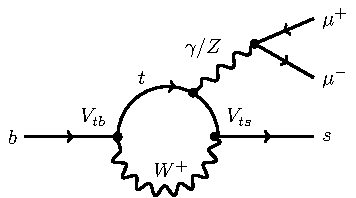
\includegraphics[scale=1]{feynman_btosmumu_penguin}
    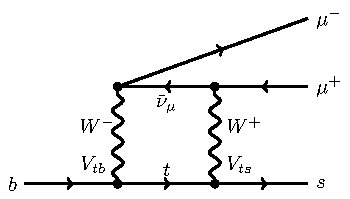
\includegraphics[scale=1]{feynman_btosmumu_box}
    \caption[Schematic Feynman diagrams for loop and box diagrams]
    {\small
      Schematic Feynman diagrams for the
      (left) penguin loop diagrams corresponding to the operators \Op{7} and \Op{9} depending on
      whether a $\gamma$ or $Z$ is emitted from the loop;
      (right) \Op{10} box diagram mediated by \Wp bosons.
    }
    \label{fig:hhh:loops}
  \end{center}
\end{figure}

The effective Hamiltonian for $\decay{b}{s\ell^+\ell^-}$ FCNCs is given by
\begin{equation}
  \Ham{eff} = -4\frac{G_F}{\sqrt{2}}\Vconj{ts}\V{tb}\frac{e^2}{16\pi^2}
  \sum_{i=1}^{10}\big[C_i(\Lambda)\mathcal{O}_i(\Lambda)
    +C_i^\prime(\Lambda)\mathcal{O}_i^\prime(\Lambda)\big],
\end{equation}
as in \Eq{eq:th:opeham}. %, where the coefficients are known as Wilson coefficients, which
%correspond to the Wilson operators $\mathcal{O}_{1-10}$.
The operators \Op{1-6} encapsulate long distance contributions, such as \ccbar
loops, and \Op{8} is the gluonic penguin operator.
Operators which are particularly sensitive to NP contributions in \decay{b}{s\mumu} transitions are
\begin{align}
  \Op{7\pz} &= \frac{m_b}{e}\big(\bar\squark\sigma_{\mu\nu}P_Rb\big)F^{\mu\nu}
  %$\bra{f}\Op}\ket{i}$.
  &\Op{7\pz}^\prime &= \frac{m_b}{e}\big(\bar s \sigma_{\mu\nu}P_Lb\big)F^{\mu\nu}
  \nonumber\\
  %\mathcal{O}_8 &= g\frac{m_b}{e^2}\big(\bar s \sigma_{\mu\nu}T^aP_Rb\big)G^{\mu\nu a}
  %&\mathcal{O}_8^\prime &= g\frac{m_b}{e^2}\big(\bar s \sigma_{\mu\nu}T^aP_Rb\big)G^{\mu\nu a}
  %\\
  \Op{9\pz} &= \big(\bar s\gamma_\mu P_Lb\big)\big(\bar\ell\gamma^\mu\ell\big)
  &\Op{9\pz}^\prime &= \big(\bar s\gamma_\mu P_Rb\big)\big(\bar\ell\gamma^\mu\ell\big)
  \nonumber\\
  \Op{10} &= \big(\bar s\gamma_\mu P_Lb\big)\big(\bar\ell\gamma^\mu\gamma_5\ell\big)
  &\Op{10}^\prime &= \big(\bar s\gamma_\mu P_Rb\big)\big(\bar\ell\gamma^\mu\gamma_5\ell\big).
  %\phantom{\frac{1}{1}}
  %\\
  %\mathcal{O}_{S} &= \frac{m_b}{m_{B_s}}\big(\bar s\gamma_\mu P_Rb\big)\big(\bar\ell\ell\big)
  %\\
  %\mathcal{O}_{P} &= \frac{m_b}{m_{B_s}}\big(\bar s\gamma_\mu P_Rb\big)\big(\bar\ell\gamma_5\ell\big)
\end{align}
The operators \Op{7} and \Op{9} describe the emission of a photon or $Z$ from a penguin loop,
and \Op{10} corresponds to a box type diagram with \Wp; these are shown in \Fig{fig:hhh:loops}.
Primed operators are the suppressed helicity, whose contributions are vanishingly small in the SM.



%%%%%%%%%%%%%%%%%%%%%%%%%%%%%%%%%%%%%%%%%%%%%%%%%%%%%%%%%%%%%%%%%%%%%%%%%%%%%%%%%%%%%%%%%%%%%%%%%%
%%%%%%%%%%%%%%%%%%%%%%%%%%%%%%%%%%%%%%%%%%%%%%%%%%%%%%%%%%%%%%%%%%%%%%%%%%%%%%%%%%%%%%%%%%%%%%%%%%




The decay \btokpipimumu can propagate as shown in \Fig{fig:hhh:feyn}, this
has similarities with the decay $\decay{\Bp}{K^*(892)^0\mumu}$.
Both propagate in the same way, but the latter's final state is $\kpi\mumu$ --- the decay
\btokpipimumu requires an additional \uubar pair.
The decay $\decay{\Bp}{K^*(892)^0\mumu}$ is of considerable interest because, not only does it
involve an FCNC, but its angular distributions are sensitive to NP.

\begin{figure}
  \begin{center}
    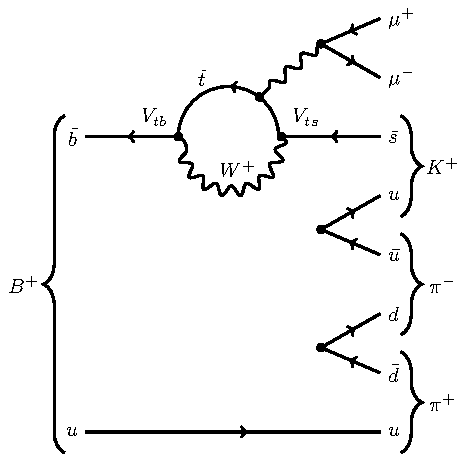
\includegraphics[scale=1]{feynman_hhh_kpipimumu}
    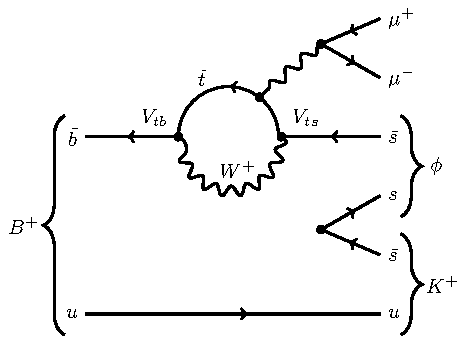
\includegraphics[scale=1]{feynman_hhh_phikmumu}
    \caption[Feynman diagrams for \btokpipimumu and \btophikmumu]
    {\small
      Feynman diagrams illustrating how the decays \btokpipimumu and \btophikmumu can proceed in
      the SM.
    }
    \label{fig:hhh:feyn}
  \end{center}
\end{figure}

The \kpipi system in the decay \btokpipimumu results from the decay of a variety of strange
resonances.
Contributions of resonances to the \kpipi system has been previously studied by the \belle
collaboration in the tree level decay \btojpsikpipi, where \jpsitomumu~\cite{Guler:2010if}.
This study indicated that the dominant contribution should be expected
to be from \decay{\kone{1270}}{\kpipi}.
The \kone{1270} meson, together with the \kone{1400}, are mass eigenstates resulting from the
mixing of the $P$-wave axial vector states $K_{1A}(1^3P_1)$ and $K_{1B}(1^1P_1)$ according to:
\begin{equation}
  \begin{pmatrix}
    \ket{\kone{1270}} \\
    \ket{\kone{1400}}
  \end{pmatrix}
  =
  \begin{pmatrix}
    \sinthetakone & \costhetakone \\
    \costhetakone & -\sinthetakone
  \end{pmatrix}
  \begin{pmatrix}
    \ket{K_{1A}^+} \\
    \ket{K_{1B}^+}
  \end{pmatrix}.
  \label{eq:k1mixing}
\end{equation}
Here, \thetakone is the mixing angle and has been measured to be both $-34^\circ$ and
$-57^\circ$~\cite{PhysRevD.47.1252,Tayduganov:2011ui,Hatanaka:2008xj,Cheng:2011pb,Divotgey:2013jba,Cheng:2013cwa}.
However, more recent measurements favour a value of
$-(34\pm13)^\circ$~\cite{Hatanaka:2008xj,Cheng:2011pb,Divotgey:2013jba,Cheng:2013cwa},
and the most recent rule out the soloution at $-57^\circ$~\cite{Divotgey:2013jba,Cheng:2013cwa}
(but with a different sign convention).



Due to the unknown composition of the $m_\kpipi$ spectrum an inclusive prediction of the branching
fraction $\BF(\btokpipimumu)$ does not exist.
However, the branching fraction of the rare decay \decay{\Bp}{\kone{1270}\mumu} is predicted to
be~\cite{Hatanaka:2008gu}
\begin{equation}
  \BF\big(\decay{\Bp}{\kone{1270}\mumu}\big) = \big(2.3\,^{+1.3}_{-1.0}\,^{+0.0}_{-0.2}\big)\e{-6},
\end{equation}
where uncertainties arise from form-factor calculations and the mixing angle, respectively.
The \kone{1270} then decays into the \kpipi final state
--- via both a non-resonant decay and various resonaces ---
with a branching fraction of
$\BF\big(\decay{\kone{1270}}{\kpipi}\big)=\big(35.7\pm3.7\big)\,\%$~\cite{PDG2012}.

Figure~\ref{fig:th:thetak1} shows the theorecitcal \qsq distribution for the decay
$\decay{\Bp}{K_1^+\mumu}$ for both the \kone{1270} and \kone{1400} and varying \thetakone.
The \decay{b}{s\mumu} can be mediated by a real photon which, for some values of \thetakone, can be
transversely polarized.
However, for some values of \thetakone the \mumu pair is fully longitudinally polarized and the
decay via a photon is forbidden.

\begin{figure}
  \begin{center}
    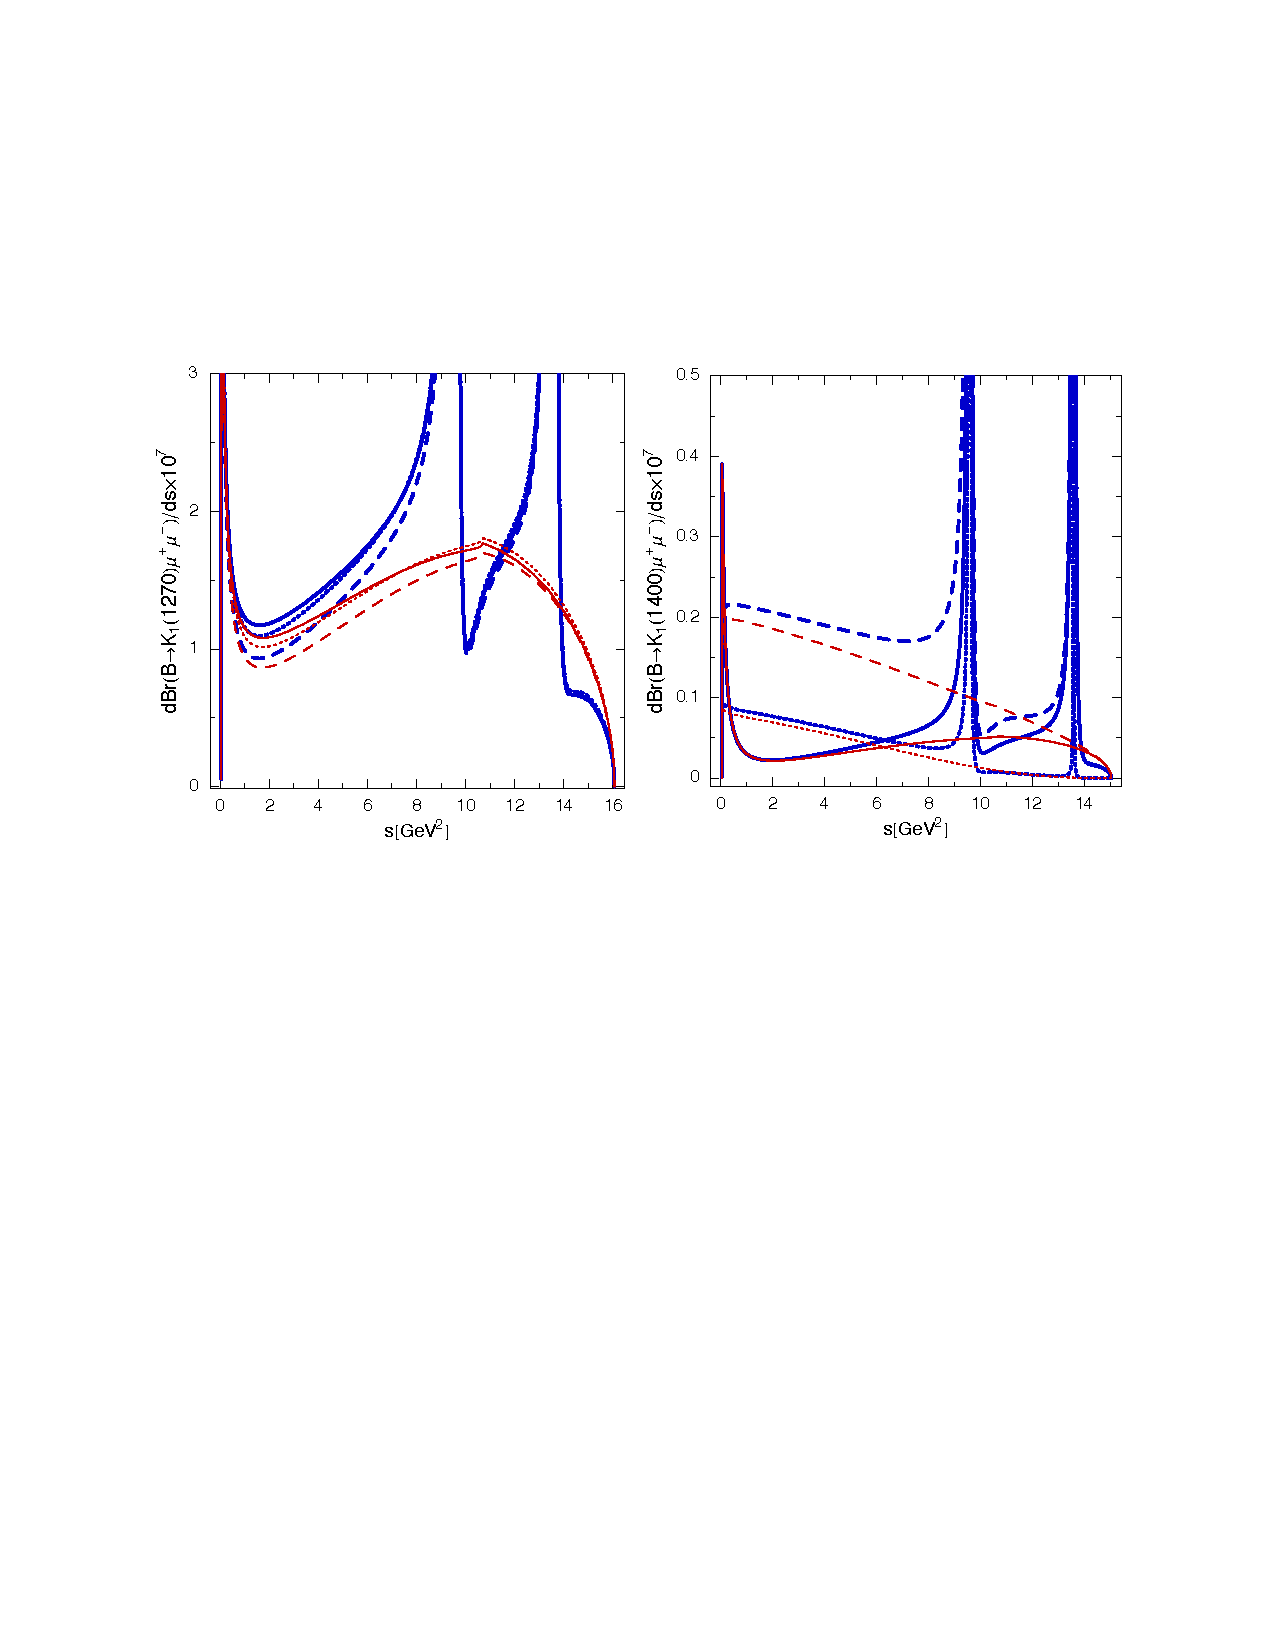
\includegraphics[width=0.96\textwidth]{K1_q2_theory}
    \caption[Theoretical \qsq distribution for $\decay{\Bp}{K_1^+\mumu}$]
    {\small
      The dimuon invariant mass distributions for the differential decay rates, as taken from
      \Ref{Hatanaka:2008gu}.
      $\dBF(\decay{\Bp}{K_1^+\mumu})/\dqsq$, (where $s=\qsq$), for the \kone{1270} and \kone{1400}.
      Central values of input form factors are used.
      The thick blue lines and thin red curves indicate the differential branching fractions with
      an without corrections from resonances, respectively.
      Solid, dotted and dashed lines correspond to values of the mixing angle
      $\thetakone=-34^\circ,-45^\circ,-57^\circ$ respectively.
    }
    \label{fig:th:thetak1}
  \end{center}
\end{figure}

The decay $\Bp\!\to\phi(1020)\Kp\mumu$ where \decay{\phi}{\kk} has no branching fraction
predictions
\footnote{All mentions of the $\phi$ meson are implicitly
  referencing the $\phi(1020)$.
}.
The expected brnahcing fraction for the decay \btophikmumu is for it to be lower with respect to
that of \btokpipimumu, because it requires an \ssbar to be \emph{popped} from the vacuum.

Absent from this analysis are the searches for the decays \decay{\Bp}{\Kp\Km\pip\mumu}
and \decay{\Bp}{\pipi\pim\mumu}.
These were not included because they are suppressed by a factor of $|\V{td}/\V{ts}|^2\simeq23$ and
suffer from large backgrounds.


\bam{The following chapter...}






%HADRONIC UNCERTAITIES
%HADROMIZAITON
